% !TeX spellcheck = en_US
\documentclass[french]{yLectureNote}

\title{Mécanique}
\subtitle{Mécanique du point}
\author{Paulhenry Saux}
\date{\today}
\yLanguage{Français}

\professor{S.Deheuvels}%sebastien.deveuhels.irap.omp.eu

\usepackage{graphicx}%----pour mettre des images
\usepackage[utf8]{inputenc}%---encodage
\usepackage{geometry}%---pour modifier les tailles et mettre a4paper
%\usepackage{awesomebox}%---pour les boites d'exercices, de pbq et de croquis ---d\'esactiv\'e pour les TP de PC
\usepackage{tikz}%---pour deiffner + d\'ependance de chemfig
\usepackage{tkz-tab}
\usepackage{chemfig}%---pour deiffner formules chimiques
\usepackage{chemformula}%---pour les formules chimiques en \'equation : \ch{...}
\usepackage{tabularx}%---pour dimensionner automatiquement les tableaux avec variable X
\usepackage{awesomebox}%---Pour les boites info, danger et autres
\usepackage{menukeys}%---Pour deiffner les touches de Calculatrice
\usepackage{fancyhdr}%---pour les en-t\^ete personnalis\'ees
\usepackage{blindtext}%---pour les liens
\usepackage{hyperref}%---pour les liens (\`a mettre en dernier)
\usepackage{caption}%---pour la francisation de la l\'egende table vers Tableau
\usepackage{pifont}
\usepackage{array}%---pour les tableaux
\usepackage{lipsum}
\usepackage{yFlatTable}
\usepackage{multicol}
\newcommand{\Lim}[1]{\lim\limits_{\substack{#1}}\:}
\renewcommand{\vec}{\overrightarrow}
\newcommand{\norm}[1]{||\vec{#1}||}
\DeclareMathOperator\arctanh{arctanh}
\begin{document}

%\titleOne
\setcounter{chapter}{4}
	\chapter{Champ électrique et magnétique }
\section{Champ vectoriel}
Pour chaque position de l'espace, $\vec{r} (= \vec{OM})$, on se donne un vecteur $\vec{u}(\vec{r},t)$. Il est appelé champ vectoriel.

Si le champ ne dépend pas du temps, il est constant. S'il ne dépend pas de l'espace, il est uniforme
\checkInfo{Exemples}{Champ de Pesanteur produit par une masse $M$ :

$\vec{F_g} = -\frac{GmM}{r^2} = m\vec{g}$ avec $\vec{g} = -\frac{GM}{r^2}$.


}
\subsection{Champ électrique}
C'est un champ vectoriel crée par une particule chargée ou bien une distribution de particules chargées.

Il s'écrit $\vec{E}(\vec{r},t)$ et s'exprime en $V\cdot m^{-1}$.
\begin{theorem}[Force électrique]
Une particule de charge $q$ plongée dans le champ $\vec{E}$ est soumise à une force $\vec{F_e} = q\times\vec{E}$.
\end{theorem}

\checkInfo{Exemples}{Le champ produit par une seule particule chargée de charge $q_0$ vaut $\frac{1}{4\pi\varepsilon_0}\frac{q_0q}{r^2}\vec{e_r} = q \times \frac{q_0}{4\pi\varepsilon_0 r^2} = q\times \vec{E}$.

Champ entre les plaques d'un condensateur : $\vec{E} = \frac{V_a-V_b}{d} \vec{e_{ab}}$. Dans le cas où les charges qui créent le champ sont immobiles dans le référentiel d'étude, on parle de champ électrostatique.
}

\subsection{Champ magnétique}
C'est aussi un champ vectoriel qui caractérise les éffets magnétiques du courant électrique ou de matérieux magnétiques par essence\marginInfo{aimants permanent, noyau de la Terre, fil parcouru par un champ électrique, Soleil} . Il est noté $\vec{B}(\vec{r},t)$ et s'exprime en Teslas, noté $T$. Le champ de la Terre est $47\mu T$.
\begin{theorem}[Force de Laplace]
La force produite par le champ vaut :$\vec{F_B} = q\vec{v} \wedge \vec{B}$
\end{theorem}
Elle est nulle si la particule est au repos ou si $\vec{v}$ et $\vec{B}$ sont colinéaires\marginTips{En effet, le produit vectoriel est alors nul et la force aussi}.
\subsection{Force magnétique + électrique}
\begin{theorem}[Force de Lorenz]
La force vaut $q\vec{E} + q\vec{v}\wedge \vec{B}$
\end{theorem}
\subsection{Ordre de grandeurs}
Faut-il prendre en compte la force de gravitation dans l'étude de la trajectoire d'une particule chargé soumise à un champ électrique et magnétique ?

Exemple : Mouvement d'un électron avec
\begin{itemize}
 \item une vitesse de 1km/s (vitesse faible)
 \item B = $10^{-4}$T
 \item E = 100 $V\cdot m^{-1}$
\end{itemize}

ODG des forces :

\begin{itemize}
 \item $F_g = mg = 10^{-30}\times 10 = 10^{-29}N$
 \item $F_e = |q|E = 10^{-19}\times 100 = 10^{-17}?$
 \item $F_b = |qV|B = 10^{-19} \times 1000 \times 10^{-4} = 10^{-20}$
\end{itemize}

Le rapport entre $F_G$ et $F_e$ donne $10^{-12} << 1$, tout comme celui entre $F_G$ et $F_b$. On peut donc négliger la force de gravitation
\section{Mouvement d'une particule chargée dans un champ électrique constant}
On considère une particule de charge $q$ initialement à l'origine avec une vitesse initiale $\vec{v_0} = V_0\vec{e_x}$, plongée dans un champ électrique uniforme et constant.

Le mouvement est dans le plan (Oxy) car pas de force selon $z$ ni de vitesse initiale.

Force : $\vec{F_e} = q\vec{E}$

On applique le PFD : $\vec{a}m = q\vec{E}$. Donc le mouvement est uniformément accéléré.

On a donc :
\[
 \left\{\begin{matrix}
 m\ddot{x} =& 0 \\
 m\ddot{y} =& qE
\end{matrix}\right.
\Rightarrow
 \left\{\begin{matrix}
 \ddot{x} =& 0\\
 \ddot{y} =& \frac{qE}{m}
\end{matrix}\right.
\]

On intègre ensuite une première fois pour obtenir la vitesse :
\[
 \left\{\begin{matrix}
 \dot{x} &= k \\
 \dot{y} &=qEt + D
\end{matrix}\right.
\Rightarrow
 \left\{\begin{matrix}
 \dot{x}(t=0) &= V_0 = k \Rightarrow k = V_0 \\
 \dot{y}-t=0) &=0 = D \Rightarrow D = 0
\end{matrix}\right.
\]
Puis une deuxième fois pour obtenir le mouvement :
\[
 \left\{\begin{matrix}
 x &= V_0t + C' \\
 y &= \frac{qE}{m}\frac{t^2}{2} + D'
\end{matrix}\right.
\Rightarrow
\left\{\begin{matrix}
 x(0) &=0 = C' \\
 y(0) &= 0 = D'
\end{matrix}\right.
\]

On obtient une trajectoire parabolique en trouvant l'équation cartésienne : $y = \frac{qE}{m}\frac{x^2}{2V_0^2}$

Le champ peut accélérer les particules.

Si $\vec{E}$ est colinéaire $ \vec{V_0}$, le mouvement est rectiligne.

Exemple : Accélérateur de particule linéaire. Longueur : 3.2 km pour des accélérations de l'odre de 6. GeV
\section{Mouvement d'une particule dans un champ magnétique constant}
\warningInfo{Nom}{On appelle ça le mouvement cyclotron.}


la force liée au champ magnétique $F_b = q\vec{B} \wedge \vec{B}$. Elle est orthogonale à $\vec{v}$ et à $\vec{B}$. Si elle uniquement soumise à $\vec{B}$.
\subsection{Analyse préliminaire}
On a : $m\vec{a} = q\vec{v}\wedge \vec{B}$.

Donc $\vec{a} \perp \vec{v}$ et le mouvement est uniforme. Donc $\norm{v} = Cst$

Donc $\vec{a}\perp\vec{B}$ Donc $\vec{a}\cdot \vec{B} = 0 \iff \frac{d \vec{v}}{dt}\cdot \vec{B} = 0$ mais B est constant, donc on a : $\frac{d}{dt} (\vec{v}\cdot\vec{B})$ puis $\frac{d}{dt}(\norm{v}\norm{B}\times\cos(\alpha))  =0$ puis $\frac{d}{dt}\cos\alpha = 0$\marginInfo{Car $\norm{v}$ et $\norm{B}$ sont constants.} donc $\alpha $ est constant. Donc l'angle entre $\vec{B}$ et $\vec{v}$ reste constant au cours du mouvement.

Exemple : Si $\vec{V_0}\perp\vec{B}$, le mouvement est dans le plan (Oxy). Car la vitesse est toujours orthogonale à $\vec{B}$.
\subsection{Étude du mouvement}
\subsubsection{On applique le PFD}

Exemple : Mouvement d'une particule dans un champ : $\vec{B} = B\vec{e_z}$ avec uniquement la force magnétique.

On a : $m\vec{a} = q\vec{v}\wedge \vec{B}$.

On fait le produit vectoriel pour trouver que
\[
 \left\{\begin{matrix}
 \ddot{x} &=qB\dot{y} \\
 \ddot{y} &=-qB\dot{x}\\
 \ddot{z} &= 0
\end{matrix}\right.
\Rightarrow
 \left\{\begin{matrix}
 \dot{v_x} &=qB\dot{v_y} \\
 \dot{v_y} &=-qB\dot{v_x}\\
\end{matrix}\right.
\]
Ce sont des EQD couplées
\subsubsection{Découplage des EQD}
On introduit la grandeur complexe $\underline{V} = V_x+iV_y$. Dans ce cas, $\underline{\dot{V}} = \dot{V_x}+i\dot{V_y}$.

On calcule $(i) + i\times (ii)$. Donc on obtient :

\begin{flalign*}
m\dot{v_x}+im\dot{v_y} &= qBV_y-iqBV_x\\
m(\dot{V_x}+i\dot{V_y}) &= qBV_y-iqBV_x\\
m(\underline{V}) &= qBV_y-iqBV_x\\
m(\underline{V}) &= -i^2qBV_y - iqBV_x\\
m(\underline{V}) &= -iqB(iV_y+V_x)\\
m(\underline{\dot{V}}) &= -iqB(\underline{V})\\
m(\underline{\dot{V}}) + iqB(\underline{V}) = 0\\
\end{flalign*}
On obtient une EQD du premier ordre linéaire à coeff constant en $\underline{V}$. On résout et on aura $V_x = Re(\underline{V})$ et $V_y = Im(\underline{V})$.

On cherche des solutions de la forme $\underline{V} = \underline{C}e^{rt}$

L'équation caractéristique donne $r = \frac{-iqB}{m}$. En posant $\omega_c$\marginCritical{C'est la pulsation cylotron, en radian/s} $= \frac{qB}{m}$, $r = -i\omega_c$ et $\underline{V} = \underline{C}e^{-i\omega_ct}$

On utilise les conditions initiales : $\vec{V_0} = V_0\vec{e_x}$, donc $\underline{V}(t=0) = V_x(0) + iV_y(0) = V_0$,

d'où $\underline{V}(t=0) =\underline{C}e^0 = \underline{C}$ et $\underline{C} = V_0$.

Donc $\underline{V}(t) = V_0e^{-i\omega_c t} = V_0(\cos(\omega_c t) - i\sin(\omega_c t)$.

Donc $V_x(t) = re(\underline{V}) = V_0\cos(\omega_c t)$ et $V_y(t) = Im(\underline{V}) = -V_0\sin(\omega_c t)$

On remarque que la vitesse reste constante et le mouvement est uniforme car $\norm{v} = \sqrt{v_x^2+v_y^2} = V_0$.

On détermine la trajectoire : on intègre pour obtenir $x(t)$ et $y(t)$.
\[
 \left\{\begin{matrix}
 x = \frac{V_0}{\omega_c}\sin(\omega_c t) + A \\
 y = \frac{V_0}{\omega_c } \cos(\omega_c t) + B\\
\end{matrix}\right.
\]

La particule est initialement en 0, donc $A=0$ et $B = \frac{-V_0}{\omega_c}$.

On obtient finalement
\[
 \left\{\begin{matrix}
 x = \frac{V_0}{\omega_c}\sin(\omega_c t)  \\
 y = \frac{V_0}{\omega_c } \cos(\omega_c t) -\frac{V_0}{\omega_c }\\
\end{matrix}\right.
\]
\checkInfo{Période de la fonction}{
Période de $x(t)$ : $\sin(w_c(t+T) = w_ct +w_cT) = \sin(w_ct)$. Donc $\omega_cT = 2\pi \iff T = \frac{2\pi}{\omega} = \frac{2m\pi}{|q|B}$.}
\subsubsection{Détermination de l'équation cartésienne}

\[
 \left\{\begin{matrix}
 x^2 = (\frac{V_0}{\omega_c})^2\sin^2(\omega_c t)  \\
 (y+\frac{V_0}{\omega_c })^2 = (\frac{V_0}{\omega_c })^2 \cos^2(\omega_c t)\\
\end{matrix}\right.
\Rightarrow
 \left\{\begin{matrix}
 x^2 + (y+\frac{V_0}{\omega_c })^2 = (\frac{V_0}{\omega_c})^2(\cos^2(\omega_c t)+\sin^2(\omega_c t)) =  (\frac{V_0}{\omega_c})^2\\
 (y+\frac{V_0}{\omega_c })^2 = (\frac{V_0}{\omega_c })^2 \cos^2(\omega_c t)\\
\end{matrix}\right.
\]

On trouve l'équation d'un cercle, de la forme $(x-x_0)^2+(y-y_0)^2 = R^2$

C'est donc une trajectoire circulaire de centre $0, -\frac{V_0}{\omega_c}$ et de rayon $\frac{V_0}{|\omega_c|}$ (car $\omega_c$ peut \^etre négative.

Représentation de la trajectoire :

\includegraphics[scale=0.5]{cm-}\includegraphics[scale=0.5]{cm+}
\section{Applications}
\subsection{Spectrométrie de masse}
\includegraphics[scale=0.5]{masse}

Rappel : champ magnétique $\vec{B}$ constant.


Un faisceau de particules de m\^eme charge $q$ arrive avec une vitesse $v_0$ initiale dans une enceinte avec $\vec{B}$ constant.

Seule la masse différencie le rayon de la trajectoire des particules de m\^eme charge


\subsection{Cyclotron}
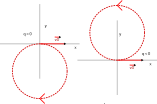
\includegraphics[scale=0.5]{cyclotron}

Accélérateur de particules : 2 enseintes demi-circulaires dans lesquels règne un champ $\vec{B}$ constant. Entre les 2 enceintes, on met en place un champ électrique $\vec{E}$

Dans les enceintes, on a une trajectoire circualire uniforme de rayon $r=\frac{Vm}{|q|B}$ (le rayon augmente avec la vitesse). Entre les enceintes, on a une trajectoire rectiligne accélérée à condition que $\vec{E}$ soit dans le sens de $\vec{v}$.

Temps mis pour faire un demi-tour ? Voir période de $x(t)$.

Il faut choisir un champ $\vec{E}$ correspondant à un courant alternatif de période $2\times T/2 = T$. La fréquence est donc $\frac{qB}{2\pi m}$.\marginInfo{Pour les vitesses $v\to c$, effets relativistes donc $m\to \gamma m = \frac{1}{\sqrt{1-\frac{v^2}{c^2}}}m$ Dans ce cas, $T_2 = \frac{\pi\gamma m}{|q|B}$.}
\end{document}

